% ============================================================================
% chain_flowchart.tex  (publication version)
% MALTA2 FMT simulation and reconstruction chain
% Compile:  pdflatex chain_flowchart.tex
% ============================================================================
\documentclass[tikz,border=6pt]{standalone}
\usepackage[T1]{fontenc}
\usepackage{lmodern}
\usetikzlibrary{positioning,arrows.meta,fit,backgrounds,calc}

% ---- palette (colorblind-safe, high-contrast print friendly) --------------
\definecolor{geantC}{RGB}{ 31,119,180}   % blue   : Monte Carlo
\definecolor{digiC}{RGB}{ 44,160, 44}    % green  : digitization
\definecolor{recoC}{RGB}{230, 97,  1}    % orange : reconstruction
\definecolor{anaC}{RGB}{123, 50,148}     % purple : analysis
\definecolor{fileG}{RGB}{ 90, 90, 90}    % slate  : intermediate data

% ---- node & arrow styles --------------------------------------------------
\tikzset{
  % Base processing box (outer width controlled strictly by minimum width)
  box/.style={
    rectangle, rounded corners=2pt, align=center, font=\small,
    minimum height=1.05cm, inner xsep=0pt, inner ysep=3pt,
    draw=black!65, line width=0.55pt
  },
  % Row-specific widths so 4-, 3-, and 2-column rows span exactly 11.50 cm
  box4/.style={box, minimum width=2.50cm, text width=2.30cm},
  box3/.style={box, minimum width=3.50cm, text width=3.30cm},
  box2/.style={box, minimum width=5.50cm, text width=5.30cm},
  % Left-hand stage badge (matches stage container height: 1.05cm + 10pt)
  lane/.style={
    rectangle, rounded corners=2pt, align=center,
    font=\small\bfseries, minimum width=3.10cm, text width=2.90cm,
    minimum height=1.05cm+10pt, inner sep=0pt, line width=0.6pt
  },
  % Shaded background container grouping each stage
  stagebox/.style={
    rectangle, rounded corners=3pt, inner sep=5pt, line width=0.6pt
  },
  % Intermediate data/file pill along the central vertical spine
  fnode/.style={
    rectangle, rounded corners=8pt, align=center, font=\small\itshape,
    minimum width=4.60cm, minimum height=0.52cm, inner sep=3pt,
    draw=fileG!80, fill=gray!10, line width=0.55pt
  },
  % Arrows: steparr for horizontal in-stage flow, dataarr for vertical spine
  steparr/.style={-{Stealth[length=2.0mm, width=1.5mm]}, semithick, draw=black!65},
  dataarr/.style={-{Stealth[length=2.3mm, width=1.8mm]}, thick, draw=black!75},
}

\begin{document}
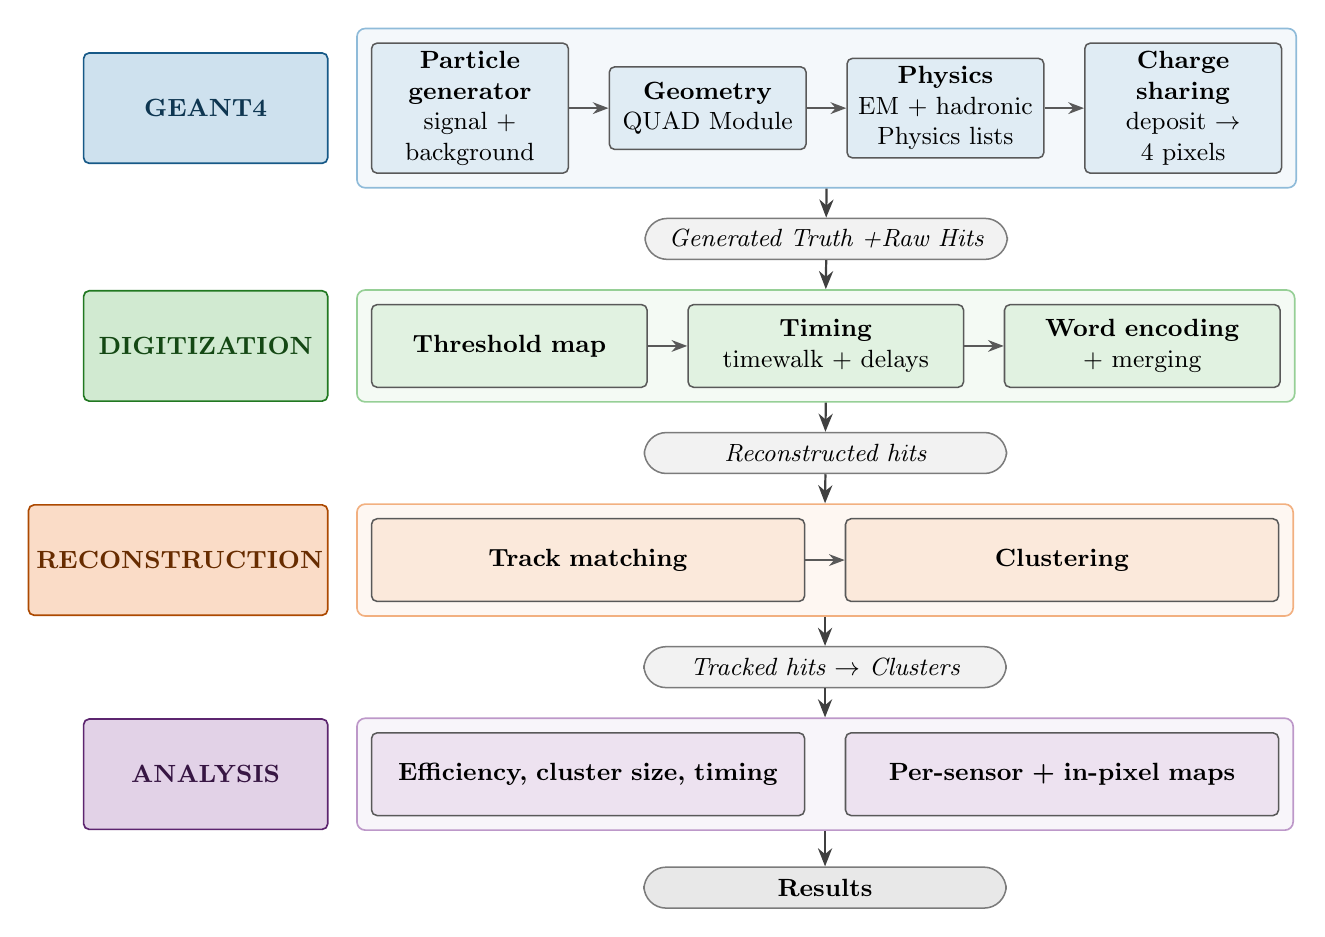
\begin{tikzpicture}[node distance=0.50cm and 0.50cm]

  % ================= LANE A : GEANT4 (4 boxes) =============================
  \node[box4, fill=geantC!14] (a1)
    {\textbf{Particle generator}\\signal + background};
  \node[box4, fill=geantC!14, right=of a1] (a2)
    {\textbf{Geometry}\\QUAD Module};
  \node[box4, fill=geantC!14, right=of a2] (a3)
    {\textbf{Physics}\\EM + hadronic Physics lists};
  \node[box4, fill=geantC!14, right=of a3] (a4)
    {\textbf{Charge sharing}\\deposit $\to$ 4 pixels};

  \draw[steparr] (a1) -- (a2);
  \draw[steparr] (a2) -- (a3);
  \draw[steparr] (a3) -- (a4);

  % ================= LANE B : DIGITIZATION (3 boxes) =======================
  \node[box3, fill=digiC!14, below=1.65cm of a1.south west, anchor=north west] (b1)
    {\textbf{Threshold map}};
  \node[box3, fill=digiC!14, right=of b1] (b2)
    {\textbf{Timing}\\timewalk + delays};
  \node[box3, fill=digiC!14, right=of b2] (b3)
    {\textbf{Word encoding}\\+ merging};

  \draw[steparr] (b1) -- (b2);
  \draw[steparr] (b2) -- (b3);

  % ================= LANE C : RECONSTRUCTION (2 boxes) =====================
  \node[box2, fill=recoC!14, below=1.65cm of b1.south west, anchor=north west] (c1)
    {\textbf{Track matching}};
  \node[box2, fill=recoC!14, right=of c1] (c2)
    {\textbf{Clustering}};

  \draw[steparr] (c1) -- (c2);

  % ================= LANE D : ANALYSIS (2 parallel boxes) ==================
  \node[box2, fill=anaC!14, below=1.65cm of c1.south west, anchor=north west] (d1)
    {\textbf{Efficiency, cluster size, timing}};
  \node[box2, fill=anaC!14, right=of d1] (d2)
    {\textbf{Per-sensor + in-pixel maps}};

  % ================= STAGE CONTAINERS (BACKGROUND LAYER) ===================
  \begin{pgfonlayer}{background}
    \node[stagebox, fill=geantC!5, draw=geantC!50, fit=(a1) (a4)] (stageA) {};
    \node[stagebox, fill=digiC!5,  draw=digiC!50,  fit=(b1) (b3)] (stageB) {};
    \node[stagebox, fill=recoC!5,  draw=recoC!50,  fit=(c1) (c2)] (stageC) {};
    \node[stagebox, fill=anaC!5,   draw=anaC!50,   fit=(d1) (d2)] (stageD) {};
  \end{pgfonlayer}

  % ================= LEFT STAGE HEADERS ====================================
  \node[lane, fill=geantC!22, draw=geantC!75!black, text=geantC!45!black,
        left=0.35cm of stageA.west] (La) {GEANT4};
  \node[lane, fill=digiC!22,  draw=digiC!75!black,  text=digiC!45!black,
        left=0.35cm of stageB.west] (Lb) {DIGITIZATION};
  \node[lane, minimum width=3.8cm, text width=3.6cm, fill=recoC!22,  draw=recoC!75!black,  text=recoC!45!black,
        left=0.35cm of stageC.west] (Lc) {RECONSTRUCTION};
  \node[lane, fill=anaC!22,   draw=anaC!75!black,   text=anaC!45!black,
        left=0.35cm of stageD.west] (Ld) {ANALYSIS};

  % ================= CENTRAL VERTICAL DATA SPINE ===========================
  \node[fnode] (fA) at ($(stageA.south)!0.5!(stageB.north)$) { Generated Truth +Raw Hits};
  \node[fnode] (fB) at ($(stageB.south)!0.5!(stageC.north)$) {Reconstructed hits};
  \node[fnode] (fC) at ($(stageC.south)!0.5!(stageD.north)$) {Tracked hits $\to$ Clusters};
  \node[fnode, below=0.45cm of stageD.south, font=\small\bfseries, fill=gray!18] (fD) {Results};

  \draw[dataarr] (stageA.south) -- (fA.north);
  \draw[dataarr] (fA.south)     -- (stageB.north);
  \draw[dataarr] (stageB.south) -- (fB.north);
  \draw[dataarr] (fB.south)     -- (stageC.north);
  \draw[dataarr] (stageC.south) -- (fC.north);
  \draw[dataarr] (fC.south)     -- (stageD.north);
  \draw[dataarr] (stageD.south) -- (fD.north);

  % ================= OPTIONAL TITLE ========================================
  % Comment out the two lines below if using a standard LaTeX \caption{} in your paper
 %% \node[font=\large\bfseries] (title)
 %%   at ($(La.north west)!0.5!(stageA.north east) + (0,0.45cm)$)
  %%  {MALTA FMT simulation and reconstruction chain};

\end{tikzpicture}
\end{document}